\documentclass[a4paper,11pt]{article}

\usepackage[T1]{fontenc}

\usepackage[utf8]{inputenc}

\usepackage[italian]{babel}

\usepackage{graphicx}

\usepackage{indentfirst}

\usepackage{amsmath,amssymb}

\usepackage{enumitem} 

\newcommand{\virgolette}[1]{``#1''}

\usepackage[margin=1in]{geometry} %Smaller margins

\usepackage{lmodern} %Vector PDF

\usepackage{siunitx}

\usepackage{xcolor}

\usepackage{colortbl}

\usepackage{booktabs}

\usepackage{graphicx}
\graphicspath{ {../Immagini/} }

\usepackage{wrapfig}

\usepackage{siunitx} % Per unit� di misura in generale e la corretta rappresentazione dei numeri.

\begin{document}

\begin{titlepage}
	\centering
	{\scshape\LARGE Laboratorio di Ottica, Elettronica e \\ Fisica Moderna \par}
	\vspace{1cm}
	{\scshape\Large Relazione di Laboratorio 5\par}
	\vspace{1.5cm}
	{\huge\bfseries Rapporto carica massa dell'elettrone\par}
	\vspace{2cm}

	{\Large\itshape Nicolò Cavalleri, Giacomo Lini e Davide Passaro
		
	(LUN12)}

	\vspace{5cm}
	\vfill

	\begin{abstract}
		Questo documento contiene la procedura e l'analisi dati di un esperimento volto a misurare il rapporto tra la carica e la massa dell'elettrone. L'esperimento seguito non corrisponde a quello di Thompson (il primo esperimento che ottenne questa misura) ma una variante che, utilizzando una coppia di bobine di Hemholtz, riesce a produrre un campo magnetico più facilmente misurabile.
	\end{abstract}


	\vfill
	{\large \today\par}
	
\end{titlepage}

\newpage

	\section{Introduzione}
	\begin{wrapfigure}{r}{0.5\textwidth}
		\centering
		\vspace{-0.5cm}
		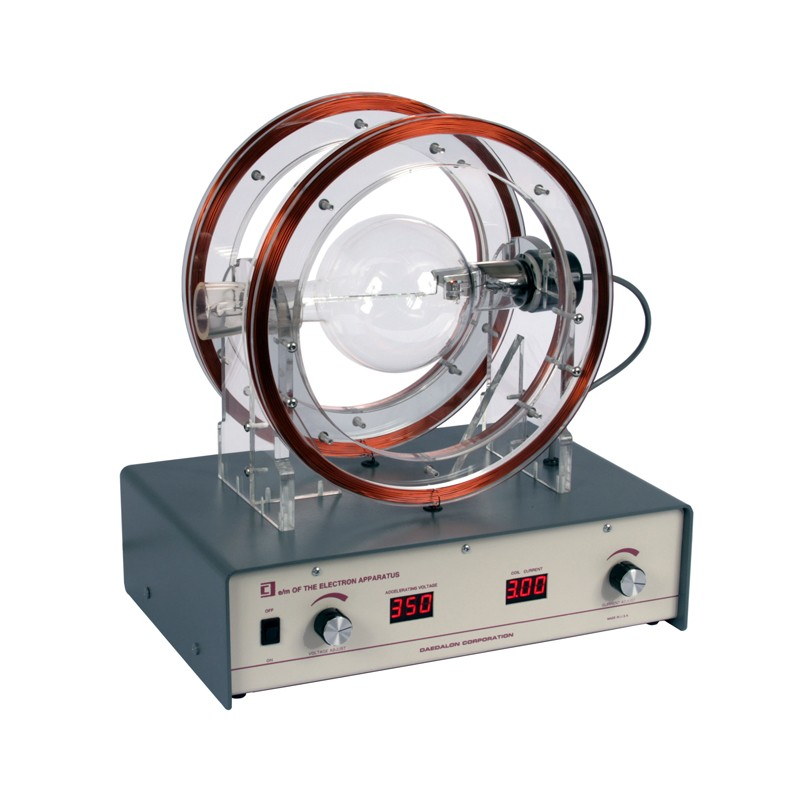
\includegraphics[width=0.5\textwidth]{apparatus}
		
		\label{apparato}
		\caption{Fotografia di un apparato simile a quello utilizzato nell'esperimento}
	\end{wrapfigure}
	L'esperimento si propone di misurare il rapporto tra la massa e la carica dell'elettrone. Questo esperimento, è stato (nella variante di J. J. Thompson) rivoluzionario per la fisica in quanto ha segnato l'inizio dello studio delle particelle fondamentali e in generale della fisica subatomica. Infatti questo esperimento provò definitivamente l'esistenza di particelle cariche negativamente (elettroni) che costituivano un argomento molto discusso e controverso anche tra i più grandi fisici dell'Ottocento. Controversie che, poco dopo, con la misura della carica dell'elettrone furono completamente risolte con la realizzazione che queste particelle avessero massa molto più piccola di quella dell'atomo di idrogeno, storicamente considerato la \virgolette{particella} più leggera esistente.
	
	In breve il procedimento seguito si è basato sulla misura della traiettoria di un fascio di elettroni sotto l'effetto di un campo elettrico ed uno magnetico. Il primo è servito per accelerare gli elettroni mentre il secondo è servito per deviare a traiettoria in un moto rettilineo uniforme di cui abbiamo facilmente calcolato il raggio.
	
	Per produrre il campo elettrico è stato utilizzato un cannone elettronico mentre per produrre il campo magnetico è stato utilizzato un sistema costituito da bobine di Hemholtz. Attraverso questi strumenti, descritti poi in seguito, siamo riusciti a creare dei campi facilmente misurabili e a modularli secondo le nostre esigenze.
	
	Infine grazie ad un'ampolla tenuta a pressione molto bassa contenente idrogeno siamo riusciti a vedere ad occhio nudo il fascio di elettroni e quindi a calcolare il raggio. 
	
	Sempre attraverso un sistema costituito da bobine di Hemholtz siamo riusciti a misurare la componente tangenziale al terreno del campo magnetico terrestre. Tutte le misure effettuate si sono rilevate compatibili con le aspettative, e nonostante molti problemi pratici descritti in seguito siamo riusciti ad ottenere delle misure abbastanza precise.
	
	
	
	
\end{document}